\documentclass[12pt,a4paper]{article}\usepackage[]{graphicx}\usepackage[]{xcolor}
% maxwidth is the original width if it is less than linewidth
% otherwise use linewidth (to make sure the graphics do not exceed the margin)
\makeatletter
\def\maxwidth{ %
  \ifdim\Gin@nat@width>\linewidth
    \linewidth
  \else
    \Gin@nat@width
  \fi
}
\makeatother

\definecolor{fgcolor}{rgb}{0.345, 0.345, 0.345}
\newcommand{\hlnum}[1]{\textcolor[rgb]{0.686,0.059,0.569}{#1}}%
\newcommand{\hlsng}[1]{\textcolor[rgb]{0.192,0.494,0.8}{#1}}%
\newcommand{\hlcom}[1]{\textcolor[rgb]{0.678,0.584,0.686}{\textit{#1}}}%
\newcommand{\hlopt}[1]{\textcolor[rgb]{0,0,0}{#1}}%
\newcommand{\hldef}[1]{\textcolor[rgb]{0.345,0.345,0.345}{#1}}%
\newcommand{\hlkwa}[1]{\textcolor[rgb]{0.161,0.373,0.58}{\textbf{#1}}}%
\newcommand{\hlkwb}[1]{\textcolor[rgb]{0.69,0.353,0.396}{#1}}%
\newcommand{\hlkwc}[1]{\textcolor[rgb]{0.333,0.667,0.333}{#1}}%
\newcommand{\hlkwd}[1]{\textcolor[rgb]{0.737,0.353,0.396}{\textbf{#1}}}%
\let\hlipl\hlkwb

\usepackage{framed}
\makeatletter
\newenvironment{kframe}{%
 \def\at@end@of@kframe{}%
 \ifinner\ifhmode%
  \def\at@end@of@kframe{\end{minipage}}%
  \begin{minipage}{\columnwidth}%
 \fi\fi%
 \def\FrameCommand##1{\hskip\@totalleftmargin \hskip-\fboxsep
 \colorbox{shadecolor}{##1}\hskip-\fboxsep
     % There is no \\@totalrightmargin, so:
     \hskip-\linewidth \hskip-\@totalleftmargin \hskip\columnwidth}%
 \MakeFramed {\advance\hsize-\width
   \@totalleftmargin\z@ \linewidth\hsize
   \@setminipage}}%
 {\par\unskip\endMakeFramed%
 \at@end@of@kframe}
\makeatother

\definecolor{shadecolor}{rgb}{.97, .97, .97}
\definecolor{messagecolor}{rgb}{0, 0, 0}
\definecolor{warningcolor}{rgb}{1, 0, 1}
\definecolor{errorcolor}{rgb}{1, 0, 0}
\newenvironment{knitrout}{}{} % an empty environment to be redefined in TeX

\usepackage{alltt}
\usepackage{mypreamble}
\usepackage{myRpreamble}
\IfFileExists{upquote.sty}{\usepackage{upquote}}{}
\begin{document}
{\bf Arkaraj Mukherjee}
{\bf Worksheet 6-2}
\\
library("tidyverse");
\begin{enumerate}[label=\arabic*.]
	\item
		\begin{enumerate}[label=(\alph*)]
			\item
			
\begin{knitrout}
\definecolor{shadecolor}{rgb}{0.969, 0.969, 0.969}\color{fgcolor}\begin{kframe}
\begin{alltt}
\hldef{corners_T} \hlkwb{=} \hlkwd{matrix}\hldef{(}\hlkwd{c}\hldef{(}\hlnum{0}\hldef{,}\hlnum{0}\hldef{,}\hlnum{1}\hldef{,}\hlnum{0}\hldef{,}\hlnum{0.5}\hldef{,}\hlkwd{sqrt}\hldef{(}\hlnum{3}\hldef{)}\hlopt{/}\hlnum{2}\hldef{),}\hlkwc{ncol} \hldef{=} \hlnum{2}\hldef{,} \hlkwc{byrow}\hldef{=}\hlnum{TRUE}\hldef{)}
\hldef{S1} \hlkwb{=} \hlkwa{function}\hldef{(} \hlkwc{point} \hldef{) \{point}\hlopt{/}\hlnum{2} \hlopt{+} \hldef{corners_T[}\hlnum{1}\hldef{,]}\hlopt{/}\hlnum{2}\hldef{\}}
\hldef{S2} \hlkwb{=} \hlkwa{function}\hldef{(} \hlkwc{point} \hldef{) \{point}\hlopt{/}\hlnum{2} \hlopt{+} \hldef{corners_T[}\hlnum{2}\hldef{,]}\hlopt{/}\hlnum{2}\hldef{\}}
\hldef{S3} \hlkwb{=} \hlkwa{function}\hldef{(} \hlkwc{point} \hldef{) \{point}\hlopt{/}\hlnum{2} \hlopt{+} \hldef{corners_T[}\hlnum{3}\hldef{,]}\hlopt{/}\hlnum{2}\hldef{\}}
\hldef{S1_set} \hlkwb{=} \hlkwa{function}\hldef{(}\hlkwc{points}\hldef{) \{}\hlkwd{t}\hldef{(}\hlkwd{apply}\hldef{(points,} \hlnum{1}\hldef{, S1))\}}
\hldef{S2_set} \hlkwb{=} \hlkwa{function}\hldef{(}\hlkwc{points}\hldef{) \{}\hlkwd{t}\hldef{(}\hlkwd{apply}\hldef{(points,} \hlnum{1}\hldef{, S2))\}}
\hldef{S3_set} \hlkwb{=} \hlkwa{function}\hldef{(}\hlkwc{points}\hldef{) \{}\hlkwd{t}\hldef{(}\hlkwd{apply}\hldef{(points,} \hlnum{1}\hldef{, S3))\}}
\hlkwd{par}\hldef{(}\hlkwc{mfrow} \hldef{=} \hlkwd{c}\hldef{(}\hlnum{1}\hldef{,}\hlnum{3}\hldef{))}
\hlkwd{plot}\hldef{(corners_T,} \hlkwc{pch} \hldef{=} \hlnum{19}\hldef{,} \hlkwc{xlab} \hldef{=} \hlsng{"x"}\hldef{,} \hlkwc{ylab} \hldef{=} \hlsng{"y"}\hldef{,} \hlkwc{main} \hldef{=} \hlsng{"under S1"}\hldef{,}\hlkwc{type} \hldef{=} \hlsng{"n"}\hldef{,}  \hlkwc{asp} \hldef{=} \hlnum{1}\hldef{)}
\hlkwd{points}\hldef{(}\hlkwd{S1_set}\hldef{(corners_T),} \hlkwc{pch} \hldef{=} \hlnum{19}\hldef{)}

\hlkwd{plot}\hldef{(corners_T,} \hlkwc{pch} \hldef{=} \hlnum{19}\hldef{,} \hlkwc{xlab} \hldef{=} \hlsng{"x"}\hldef{,} \hlkwc{ylab} \hldef{=} \hlsng{"y"}\hldef{,} \hlkwc{main} \hldef{=} \hlsng{"under S2"}\hldef{,} \hlkwc{type} \hldef{=} \hlsng{"n"}\hldef{,} \hlkwc{asp} \hldef{=} \hlnum{1}\hldef{)}
\hlkwd{points}\hldef{(}\hlkwd{S2_set}\hldef{(corners_T),} \hlkwc{pch} \hldef{=} \hlnum{19}\hldef{)}

\hlkwd{plot}\hldef{(corners_T,} \hlkwc{pch} \hldef{=} \hlnum{19}\hldef{,} \hlkwc{xlab} \hldef{=} \hlsng{"x"}\hldef{,} \hlkwc{ylab} \hldef{=} \hlsng{"y"}\hldef{,} \hlkwc{main} \hldef{=} \hlsng{"under S3"}\hldef{,} \hlkwc{type} \hldef{=} \hlsng{"n"}\hldef{,} \hlkwc{asp} \hldef{=} \hlnum{1}\hldef{)}
\hlkwd{points}\hldef{(}\hlkwd{S3_set}\hldef{(corners_T),} \hlkwc{pch} \hldef{=} \hlnum{19}\hldef{)}
\end{alltt}
\end{kframe}
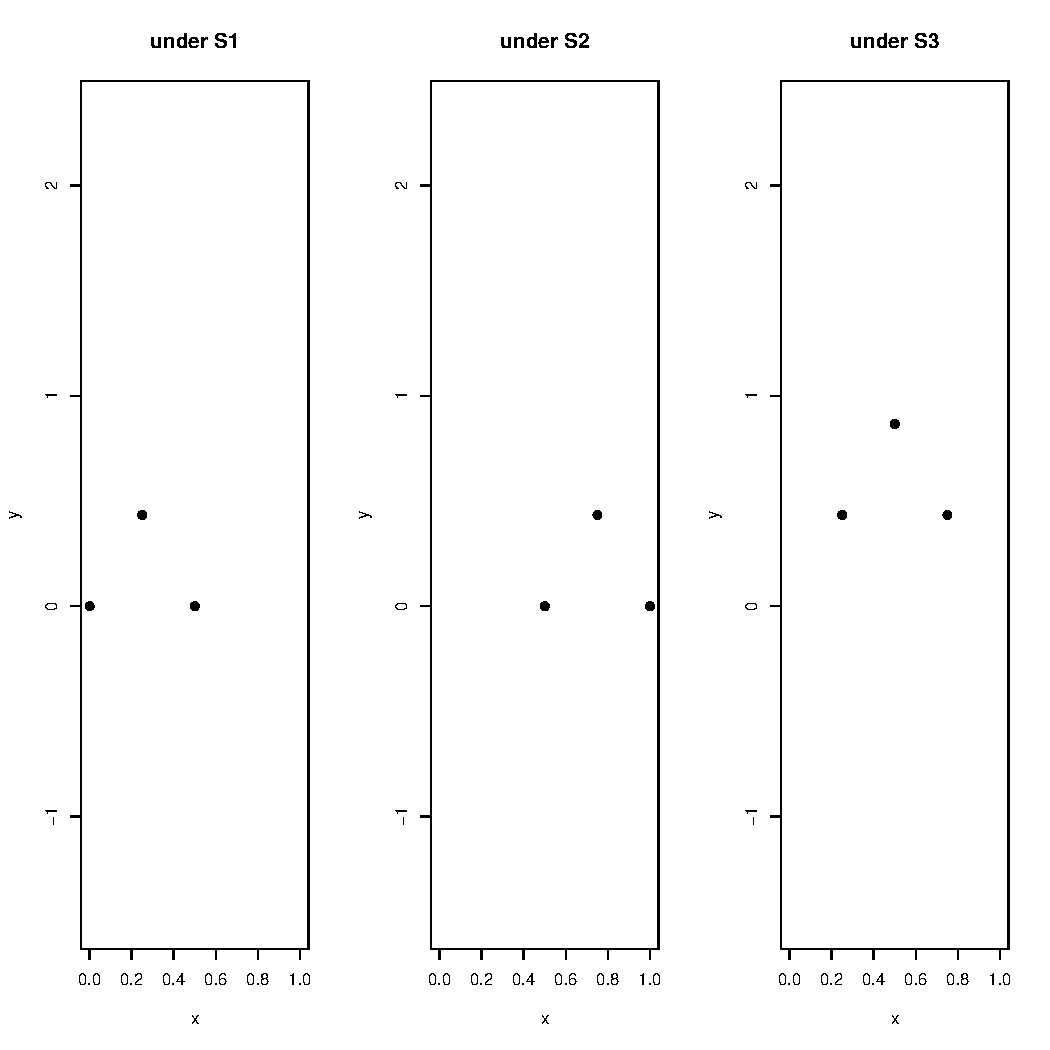
\includegraphics[width=\maxwidth]{figure/unnamed-chunk-1-1} 
\end{knitrout}
			\item
\begin{knitrout}
\definecolor{shadecolor}{rgb}{0.969, 0.969, 0.969}\color{fgcolor}\begin{kframe}
\begin{alltt}
\hldef{points_on_line} \hlkwb{<-} \hlkwa{function}\hldef{(}\hlkwc{a}\hldef{,} \hlkwc{b}\hldef{)}
\hldef{\{}
  \hldef{lam} \hlkwb{<-} \hlkwd{seq}\hldef{(}\hlnum{0}\hldef{,} \hlnum{1}\hldef{,} \hlkwc{length} \hldef{=} \hlnum{50}\hldef{)}
  \hlkwd{t}\hldef{(}\hlkwd{sapply}\hldef{(lam,} \hlkwa{function}\hldef{(}\hlkwc{l}\hldef{) l}\hlopt{*}\hldef{a} \hlopt{+} \hldef{(}\hlnum{1}\hlopt{-}\hldef{l)}\hlopt{*}\hldef{b))}
\hldef{\}}
\hldef{l1} \hlkwb{<-} \hlkwd{points_on_line}\hldef{(corners_T[}\hlnum{1}\hldef{,], corners_T[}\hlnum{2}\hldef{, ])}
\hldef{l2} \hlkwb{<-} \hlkwd{points_on_line}\hldef{(corners_T[}\hlnum{1}\hldef{,], corners_T[}\hlnum{3}\hldef{, ])}
\hldef{l3} \hlkwb{<-} \hlkwd{points_on_line}\hldef{(corners_T[}\hlnum{2}\hldef{,], corners_T[}\hlnum{3}\hldef{, ])}
\hldef{edges_T} \hlkwb{<-} \hlkwd{rbind}\hldef{(l1, l2, l3)}
\hldef{S1_edges} \hlkwb{<-} \hlkwd{S1_set}\hldef{(edges_T)}
\hldef{S2_edges} \hlkwb{<-} \hlkwd{S2_set}\hldef{(edges_T)}
\hldef{S3_edges} \hlkwb{<-} \hlkwd{S3_set}\hldef{(edges_T)}
\hlkwd{par}\hldef{(}\hlkwc{mfrow} \hldef{=} \hlkwd{c}\hldef{(}\hlnum{1}\hldef{,}\hlnum{3}\hldef{))}
\hlkwd{plot}\hldef{(edges_T,} \hlkwc{pch} \hldef{=} \hlnum{19}\hldef{,} \hlkwc{xlab} \hldef{=} \hlsng{"x"}\hldef{,} \hlkwc{ylab} \hldef{=} \hlsng{"y"}\hldef{,}
     \hlkwc{main} \hldef{=} \hlsng{"S1(edges)"}\hldef{,} \hlkwc{type} \hldef{=} \hlsng{"n"}\hldef{,} \hlkwc{asp} \hldef{=} \hlnum{1}\hldef{)}
\hlkwd{points}\hldef{(S1_edges,} \hlkwc{pch} \hldef{=} \hlnum{19}\hldef{)}
\hlkwd{plot}\hldef{(edges_T,} \hlkwc{pch} \hldef{=} \hlnum{19}\hldef{,} \hlkwc{xlab} \hldef{=} \hlsng{"x"}\hldef{,} \hlkwc{ylab} \hldef{=} \hlsng{"y"}\hldef{,}
     \hlkwc{main} \hldef{=} \hlsng{"S2(edges)"}\hldef{,} \hlkwc{type} \hldef{=} \hlsng{"n"}\hldef{,} \hlkwc{asp} \hldef{=} \hlnum{1}\hldef{)}
\hlkwd{points}\hldef{(S2_edges,} \hlkwc{pch} \hldef{=} \hlnum{19}\hldef{)}
\hlkwd{plot}\hldef{(edges_T,} \hlkwc{pch} \hldef{=} \hlnum{19}\hldef{,} \hlkwc{xlab} \hldef{=} \hlsng{"x"}\hldef{,} \hlkwc{ylab} \hldef{=} \hlsng{"y"}\hldef{,}
     \hlkwc{main} \hldef{=} \hlsng{"S3(edges)"}\hldef{,} \hlkwc{type} \hldef{=} \hlsng{"n"}\hldef{)}
\hlkwd{points}\hldef{(S3_edges,} \hlkwc{pch} \hldef{=} \hlnum{19}\hldef{)}
\end{alltt}
\end{kframe}
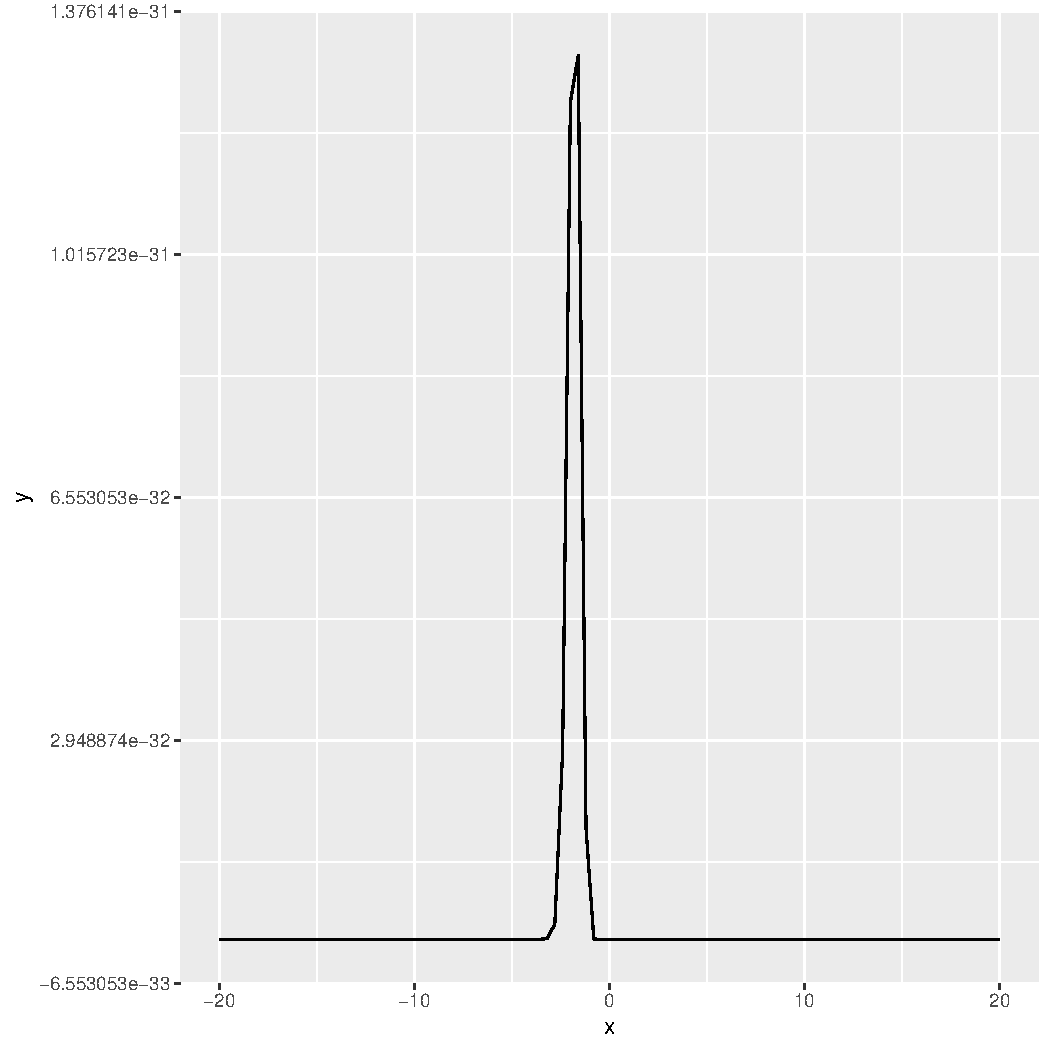
\includegraphics[width=\maxwidth]{figure/unnamed-chunk-2-1} 
\end{knitrout}
	\end{enumerate}
			\begin{enumerate}[label=(\alph*)]
			\item
\begin{knitrout}
\definecolor{shadecolor}{rgb}{0.969, 0.969, 0.969}\color{fgcolor}\begin{kframe}
\begin{alltt}
\hldef{iterative_func} \hlkwb{<-} \hlkwa{function}\hldef{(}\hlkwc{set}\hldef{)} \hlkwd{rbind}\hldef{(}\hlkwd{S1_set}\hldef{(set),} \hlkwd{S2_set}\hldef{(set),} \hlkwd{S3_set}\hldef{(set))}

\hldef{T0} \hlkwb{<-} \hldef{corners_T}
\hldef{T1} \hlkwb{<-} \hlkwd{iterative_func}\hldef{(T0)}
\hldef{T2} \hlkwb{<-} \hlkwd{iterative_func}\hldef{(T1)}
\hldef{T3} \hlkwb{<-} \hlkwd{iterative_func}\hldef{(T2)}
\hldef{T4} \hlkwb{<-} \hlkwd{iterative_func}\hldef{(T3)}
\hldef{T5} \hlkwb{<-} \hlkwd{iterative_func}\hldef{(T4)}

\hlkwd{par}\hldef{(}\hlkwc{mfrow} \hldef{=} \hlkwd{c}\hldef{(}\hlnum{2}\hldef{,}\hlnum{3}\hldef{))}
\hlkwd{plot}\hldef{(T0,} \hlkwc{pch} \hldef{=} \hlnum{20}\hldef{,} \hlkwc{cex} \hldef{=} \hlnum{0.5}\hldef{,} \hlkwc{main} \hldef{=} \hlsng{"T0"}\hldef{,} \hlkwc{asp} \hldef{=} \hlnum{1}\hldef{)}
\hlkwd{plot}\hldef{(T1,} \hlkwc{col} \hldef{=} \hlnum{2}\hldef{,} \hlkwc{pch} \hldef{=} \hlnum{20}\hldef{,} \hlkwc{cex} \hldef{=} \hlnum{0.5}\hldef{,} \hlkwc{main} \hldef{=} \hlsng{"T1"}\hldef{,} \hlkwc{asp} \hldef{=} \hlnum{1}\hldef{)}
\hlkwd{plot}\hldef{(T2,} \hlkwc{col} \hldef{=} \hlnum{3}\hldef{,} \hlkwc{pch} \hldef{=} \hlnum{20}\hldef{,} \hlkwc{cex} \hldef{=} \hlnum{0.5}\hldef{,} \hlkwc{main} \hldef{=} \hlsng{"T2"}\hldef{,} \hlkwc{asp} \hldef{=} \hlnum{1}\hldef{)}
\hlkwd{plot}\hldef{(T3,} \hlkwc{col} \hldef{=} \hlnum{4}\hldef{,} \hlkwc{pch} \hldef{=} \hlnum{20}\hldef{,} \hlkwc{cex} \hldef{=} \hlnum{0.5}\hldef{,} \hlkwc{main} \hldef{=} \hlsng{"T3"}\hldef{,} \hlkwc{asp} \hldef{=} \hlnum{1}\hldef{)}
\hlkwd{plot}\hldef{(T4,} \hlkwc{col} \hldef{=} \hlnum{5}\hldef{,} \hlkwc{pch} \hldef{=} \hlnum{20}\hldef{,} \hlkwc{cex} \hldef{=} \hlnum{0.5}\hldef{,} \hlkwc{main} \hldef{=} \hlsng{"T4"}\hldef{,} \hlkwc{asp} \hldef{=} \hlnum{1}\hldef{)}
\hlkwd{plot}\hldef{(T5,} \hlkwc{col} \hldef{=} \hlnum{6}\hldef{,} \hlkwc{pch} \hldef{=} \hlnum{20}\hldef{,} \hlkwc{cex} \hldef{=} \hlnum{0.5}\hldef{,} \hlkwc{main} \hldef{=} \hlsng{"T5"}\hldef{,} \hlkwc{asp} \hldef{=} \hlnum{1}\hldef{)}
\end{alltt}
\end{kframe}
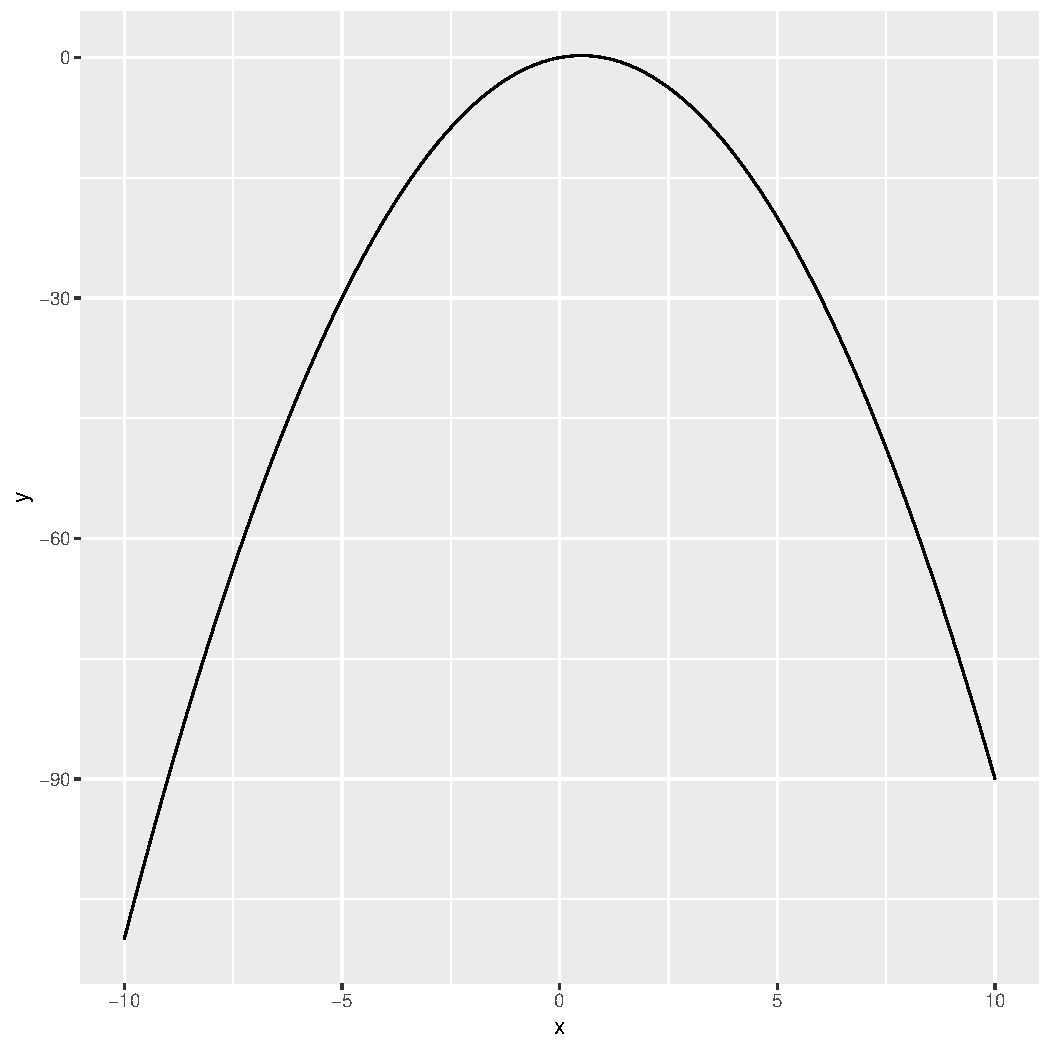
\includegraphics[width=\maxwidth]{figure/unnamed-chunk-3-1} 
\end{knitrout}
		\item Yes, they are contained in all the iterationss.
		\item
\begin{knitrout}
\definecolor{shadecolor}{rgb}{0.969, 0.969, 0.969}\color{fgcolor}\begin{kframe}
\begin{alltt}
\hldef{T0} \hlkwb{<-} \hldef{edges_T}
\hldef{T1} \hlkwb{<-} \hlkwd{iterative_func}\hldef{(T0)}
\hldef{T2} \hlkwb{<-} \hlkwd{iterative_func}\hldef{(T1)}
\hldef{T3} \hlkwb{<-} \hlkwd{iterative_func}\hldef{(T2)}
\hldef{T4} \hlkwb{<-} \hlkwd{iterative_func}\hldef{(T3)}
\hldef{T5} \hlkwb{<-} \hlkwd{iterative_func}\hldef{(T4)}

\hlkwd{par}\hldef{(}\hlkwc{mfrow} \hldef{=} \hlkwd{c}\hldef{(}\hlnum{2}\hldef{,}\hlnum{3}\hldef{))}
\hlkwd{plot}\hldef{(T0,} \hlkwc{pch} \hldef{=} \hlnum{20}\hldef{,} \hlkwc{cex} \hldef{=} \hlnum{0.1}\hldef{,} \hlkwc{main} \hldef{=} \hlsng{"T0 (Edges)"}\hldef{,} \hlkwc{asp} \hldef{=} \hlnum{1}\hldef{)}
\hlkwd{plot}\hldef{(T1,} \hlkwc{col} \hldef{=} \hlnum{2}\hldef{,} \hlkwc{pch} \hldef{=} \hlnum{20}\hldef{,} \hlkwc{cex} \hldef{=} \hlnum{0.1}\hldef{,} \hlkwc{main} \hldef{=} \hlsng{"T1"}\hldef{,} \hlkwc{asp} \hldef{=} \hlnum{1}\hldef{)}
\hlkwd{plot}\hldef{(T2,} \hlkwc{col} \hldef{=} \hlnum{3}\hldef{,} \hlkwc{pch} \hldef{=} \hlnum{20}\hldef{,} \hlkwc{cex} \hldef{=} \hlnum{0.1}\hldef{,} \hlkwc{main} \hldef{=} \hlsng{"T2"}\hldef{,} \hlkwc{asp} \hldef{=} \hlnum{1}\hldef{)}
\hlkwd{plot}\hldef{(T3,} \hlkwc{col} \hldef{=} \hlnum{4}\hldef{,} \hlkwc{pch} \hldef{=} \hlnum{20}\hldef{,} \hlkwc{cex} \hldef{=} \hlnum{0.1}\hldef{,} \hlkwc{main} \hldef{=} \hlsng{"T3"}\hldef{,} \hlkwc{asp} \hldef{=} \hlnum{1}\hldef{)}
\hlkwd{plot}\hldef{(T4,} \hlkwc{col} \hldef{=} \hlnum{5}\hldef{,} \hlkwc{pch} \hldef{=} \hlnum{20}\hldef{,} \hlkwc{cex} \hldef{=} \hlnum{0.1}\hldef{,} \hlkwc{main} \hldef{=} \hlsng{"T4"}\hldef{,} \hlkwc{asp} \hldef{=} \hlnum{1}\hldef{)}
\hlkwd{plot}\hldef{(T5,} \hlkwc{col} \hldef{=} \hlnum{6}\hldef{,} \hlkwc{pch} \hldef{=} \hlnum{20}\hldef{,} \hlkwc{cex} \hldef{=} \hlnum{0.1}\hldef{,} \hlkwc{main} \hldef{=} \hlsng{"T5"}\hldef{,} \hlkwc{asp} \hldef{=} \hlnum{1}\hldef{)}
\end{alltt}
\end{kframe}
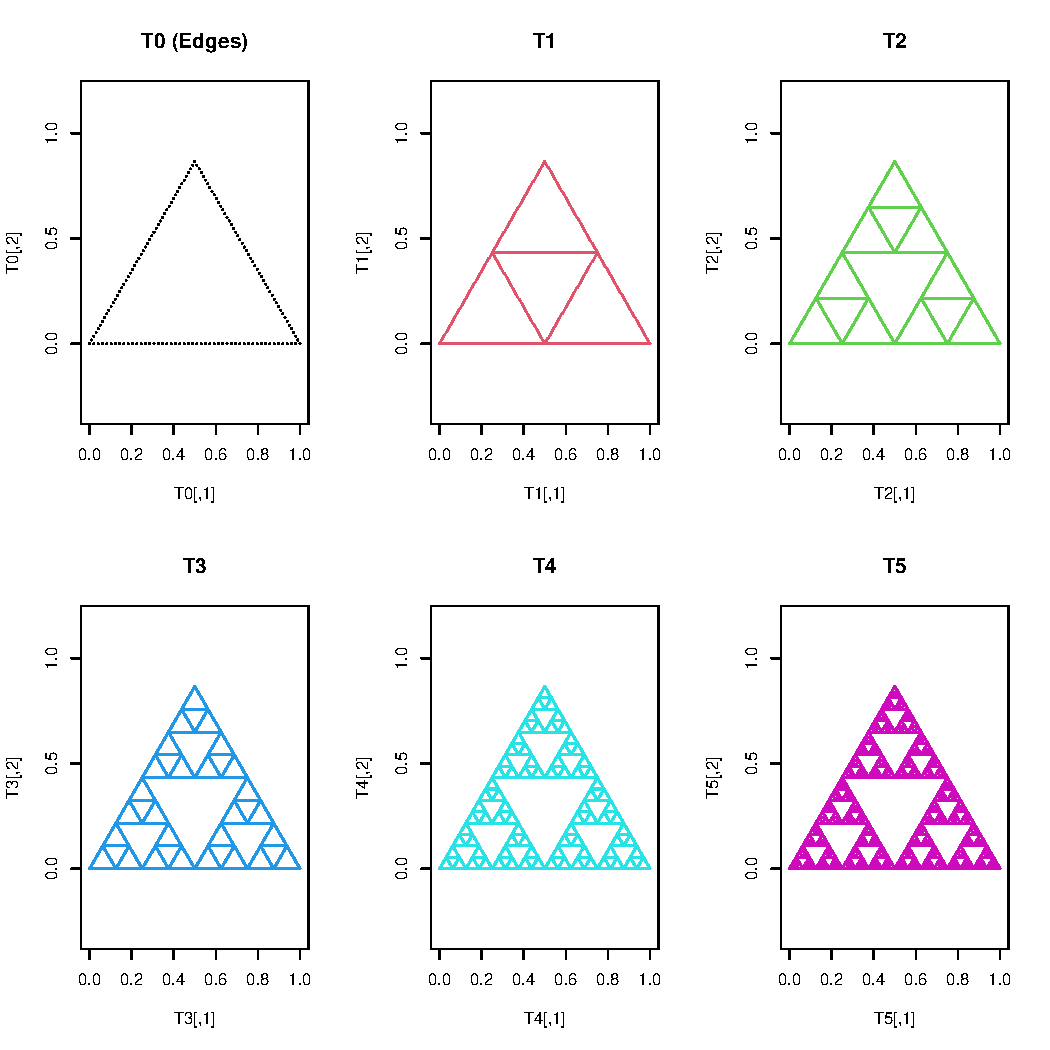
\includegraphics[width=\maxwidth]{figure/unnamed-chunk-4-1} 
\end{knitrout}
		\item
\begin{knitrout}
\definecolor{shadecolor}{rgb}{0.969, 0.969, 0.969}\color{fgcolor}\begin{kframe}
\begin{alltt}
\hldef{filling_T} \hlkwb{<-} \hlkwa{function}\hldef{(}\hlkwc{a}\hldef{,} \hlkwc{b}\hldef{,} \hlkwc{c}\hldef{)}
\hldef{\{}
  \hldef{points} \hlkwb{<-} \hlkwa{NULL}
  \hldef{lam1} \hlkwb{<-} \hlkwd{seq}\hldef{(}\hlnum{0}\hldef{,} \hlnum{1}\hldef{,} \hlkwc{length} \hldef{=} \hlnum{25}\hldef{)}
  \hldef{lam2} \hlkwb{<-} \hlkwd{seq}\hldef{(}\hlnum{0}\hldef{,} \hlnum{1}\hldef{,} \hlkwc{length} \hldef{=} \hlnum{25}\hldef{)}
  \hlkwa{for}\hldef{(l1} \hlkwa{in} \hldef{lam1)}
  \hldef{\{}
    \hlkwa{for}\hldef{(l2} \hlkwa{in} \hldef{lam2)}
    \hldef{\{}
      \hlkwa{if}\hldef{(l1} \hlopt{+} \hldef{l2} \hlopt{<} \hlnum{1}\hldef{) points} \hlkwb{<-} \hlkwd{rbind}\hldef{(points, l1}\hlopt{*}\hldef{a} \hlopt{+} \hldef{l2}\hlopt{*}\hldef{b} \hlopt{+} \hldef{(}\hlnum{1} \hlopt{-} \hldef{l1} \hlopt{-} \hldef{l2)}\hlopt{*}\hldef{c)}
    \hldef{\}}
  \hldef{\}}
  \hldef{points}
\hldef{\}}

\hldef{points_T} \hlkwb{<-} \hlkwd{filling_T}\hldef{(corners_T[}\hlnum{1}\hldef{,], corners_T[}\hlnum{2}\hldef{, ], corners_T[}\hlnum{3}\hldef{, ])}

\hldef{T0} \hlkwb{<-} \hldef{points_T}
\hldef{T1} \hlkwb{<-} \hlkwd{iterative_func}\hldef{(T0)}
\hldef{T2} \hlkwb{<-} \hlkwd{iterative_func}\hldef{(T1)}
\hldef{T3} \hlkwb{<-} \hlkwd{iterative_func}\hldef{(T2)}
\hldef{T4} \hlkwb{<-} \hlkwd{iterative_func}\hldef{(T3)}
\hldef{T5} \hlkwb{<-} \hlkwd{iterative_func}\hldef{(T4)}

\hlkwd{par}\hldef{(}\hlkwc{mfrow} \hldef{=} \hlkwd{c}\hldef{(}\hlnum{2}\hldef{,}\hlnum{3}\hldef{))}
\hlkwd{plot}\hldef{(T0,} \hlkwc{pch} \hldef{=} \hlnum{20}\hldef{,} \hlkwc{cex} \hldef{=} \hlnum{0.01}\hldef{,} \hlkwc{main} \hldef{=} \hlsng{"T0 (Filled (not really, many points actually)"}\hldef{,} \hlkwc{asp} \hldef{=} \hlnum{1}\hldef{)}
\hlkwd{plot}\hldef{(T1,} \hlkwc{col} \hldef{=} \hlnum{2}\hldef{,} \hlkwc{pch} \hldef{=} \hlnum{20}\hldef{,} \hlkwc{cex} \hldef{=} \hlnum{0.01}\hldef{,} \hlkwc{main} \hldef{=} \hlsng{"T1"}\hldef{,} \hlkwc{asp} \hldef{=} \hlnum{1}\hldef{)}
\hlkwd{plot}\hldef{(T2,} \hlkwc{col} \hldef{=} \hlnum{3}\hldef{,} \hlkwc{pch} \hldef{=} \hlnum{20}\hldef{,} \hlkwc{cex} \hldef{=} \hlnum{0.01}\hldef{,} \hlkwc{main} \hldef{=} \hlsng{"T2"}\hldef{,} \hlkwc{asp} \hldef{=} \hlnum{1}\hldef{)}
\hlkwd{plot}\hldef{(T3,} \hlkwc{col} \hldef{=} \hlnum{4}\hldef{,} \hlkwc{pch} \hldef{=} \hlnum{20}\hldef{,} \hlkwc{cex} \hldef{=} \hlnum{0.01}\hldef{,} \hlkwc{main} \hldef{=} \hlsng{"T3"}\hldef{,} \hlkwc{asp} \hldef{=} \hlnum{1}\hldef{)}
\hlkwd{plot}\hldef{(T4,} \hlkwc{col} \hldef{=} \hlnum{5}\hldef{,} \hlkwc{pch} \hldef{=} \hlnum{20}\hldef{,} \hlkwc{cex} \hldef{=} \hlnum{0.01}\hldef{,} \hlkwc{main} \hldef{=} \hlsng{"T4"}\hldef{,} \hlkwc{asp} \hldef{=} \hlnum{1}\hldef{)}
\hlkwd{plot}\hldef{(T5,} \hlkwc{col} \hldef{=} \hlnum{6}\hldef{,} \hlkwc{pch} \hldef{=} \hlnum{20}\hldef{,} \hlkwc{cex} \hldef{=} \hlnum{0.01}\hldef{,} \hlkwc{main} \hldef{=} \hlsng{"T5"}\hldef{,} \hlkwc{asp} \hldef{=} \hlnum{1}\hldef{)}
\end{alltt}
\end{kframe}
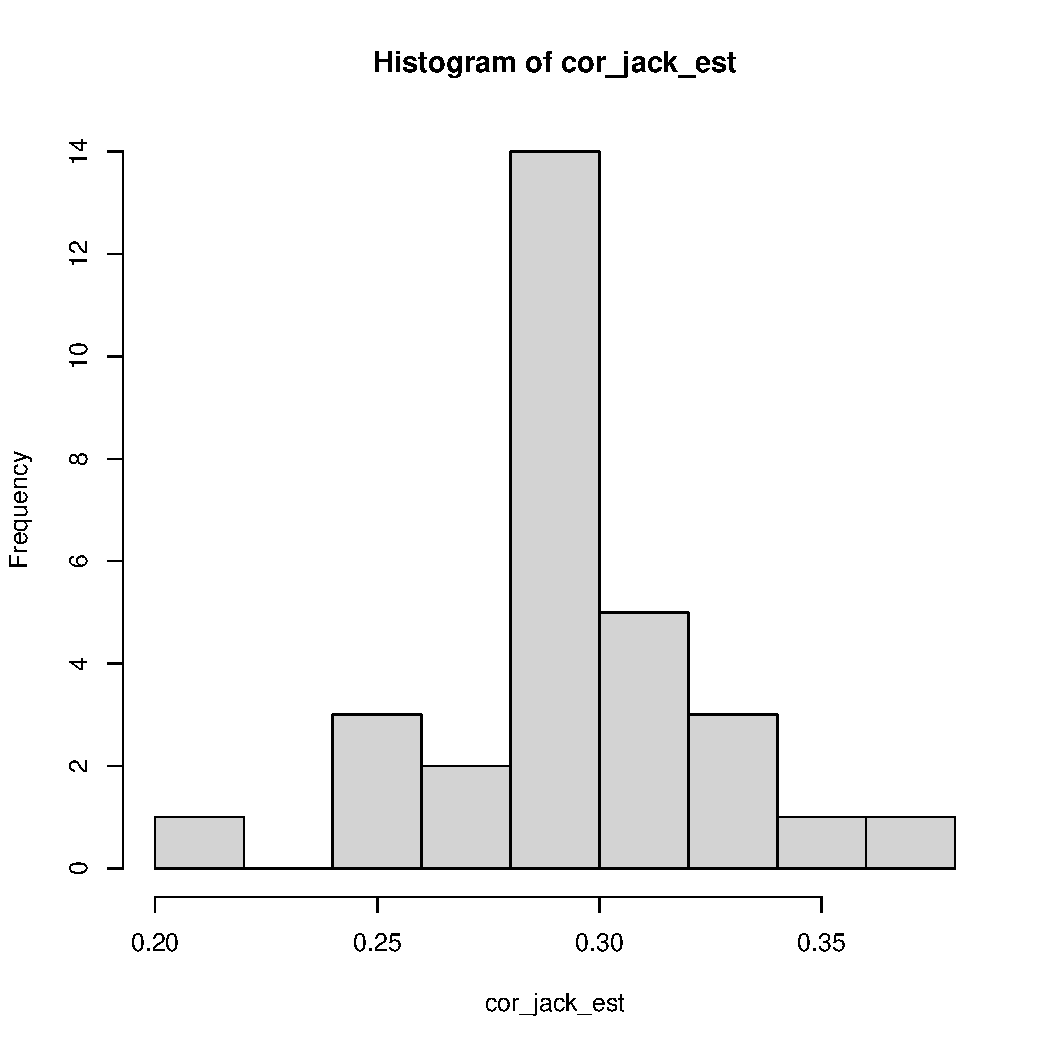
\includegraphics[width=\maxwidth]{figure/unnamed-chunk-5-1} 
\end{knitrout}
			I can not spot any difference but there is a difference between these theoretically, the removed triangles are way too small to be seen in the window I have the pdf reader open in, its half my screen for reference.
		\end{enumerate}
	\item\begin{enumerate}[label=(\alph*)]
			\item 
\begin{knitrout}
\definecolor{shadecolor}{rgb}{0.969, 0.969, 0.969}\color{fgcolor}\begin{kframe}
\begin{alltt}
\hldef{affine_map} \hlkwb{=} \hlkwa{function}\hldef{(}\hlkwc{x}\hldef{,} \hlkwc{h}\hldef{,} \hlkwc{centroid}\hldef{,} \hlkwc{theta}\hldef{)}
\hldef{\{}
  \hldef{c_old} \hlkwb{=} \hlkwd{matrix}\hldef{(}\hlkwd{c}\hldef{(}\hlnum{0.5}\hldef{,} \hlnum{1}\hlopt{/}\hldef{(}\hlnum{2}\hlopt{*}\hlkwd{sqrt}\hldef{(}\hlnum{3}\hldef{))),} \hlkwc{ncol} \hldef{=} \hlnum{1}\hldef{)}
  \hldef{Rot_mat} \hlkwb{=} \hlkwd{matrix}\hldef{(}\hlkwd{c}\hldef{(}\hlkwd{cos}\hldef{(theta),} \hlkwd{sin}\hldef{(theta),} \hlopt{-}\hlkwd{sin}\hldef{(theta),} \hlkwd{cos}\hldef{(theta)),} \hlkwc{nrow} \hldef{=} \hlnum{2}\hldef{,} \hlkwc{ncol} \hldef{=} \hlnum{2}\hldef{)}
  \hldef{x_vec} \hlkwb{=} \hlkwd{matrix}\hldef{(x,} \hlkwc{ncol} \hldef{=} \hlnum{1}\hldef{)}
  \hldef{c_new} \hlkwb{=} \hlkwd{matrix}\hldef{(centroid,} \hlkwc{ncol} \hldef{=} \hlnum{1}\hldef{)}
  \hldef{u} \hlkwb{=} \hldef{c_new} \hlopt{-} \hldef{h} \hlopt{*} \hldef{(Rot_mat} \hlopt{%*%} \hldef{c_old)}
  \hlkwd{as.vector}\hldef{(h} \hlopt{*} \hldef{(Rot_mat} \hlopt{%*%} \hldef{x_vec)} \hlopt{+} \hldef{u)}
\hldef{\}}
\end{alltt}
\end{kframe}
\end{knitrout}
		\item
\begin{knitrout}
\definecolor{shadecolor}{rgb}{0.969, 0.969, 0.969}\color{fgcolor}\begin{kframe}
\begin{alltt}
\hlkwd{par}\hldef{(}\hlkwc{mfrow} \hldef{=} \hlkwd{c}\hldef{(}\hlnum{1}\hldef{,}\hlnum{2}\hldef{))}
\hldef{T5_a} \hlkwb{<-} \hlkwd{t}\hldef{(}\hlkwd{apply}\hldef{(T5,} \hlnum{1}\hldef{,} \hlkwa{function}\hldef{(}\hlkwc{p}\hldef{)} \hlkwd{affine_map}\hldef{(p,} \hlnum{1}\hldef{,} \hlkwd{c}\hldef{(}\hlnum{0}\hldef{,}\hlnum{0}\hldef{),} \hlnum{0}\hldef{)))}
\hlkwd{plot}\hldef{(T5_a,} \hlkwc{col} \hldef{=} \hlnum{2}\hldef{,} \hlkwc{pch} \hldef{=} \hlnum{20}\hldef{,} \hlkwc{cex} \hldef{=} \hlnum{0.01}\hldef{,} \hlkwc{asp} \hldef{=} \hlnum{1}\hldef{)}

\hldef{T5_b} \hlkwb{<-} \hlkwd{t}\hldef{(}\hlkwd{apply}\hldef{(T5,} \hlnum{1}\hldef{,} \hlkwa{function}\hldef{(}\hlkwc{p}\hldef{)} \hlkwd{affine_map}\hldef{(p,} \hlnum{0.5}\hldef{,} \hlkwd{c}\hldef{(}\hlnum{5}\hldef{,}\hlnum{3}\hldef{), pi}\hlopt{/}\hlnum{6}\hldef{)))}
\hlkwd{plot}\hldef{(T5_b,} \hlkwc{col} \hldef{=} \hlnum{2}\hldef{,} \hlkwc{pch} \hldef{=} \hlnum{20}\hldef{,} \hlkwc{cex} \hldef{=} \hlnum{0.01}\hldef{,} \hlkwc{asp} \hldef{=} \hlnum{1}\hldef{)}
\end{alltt}
\end{kframe}
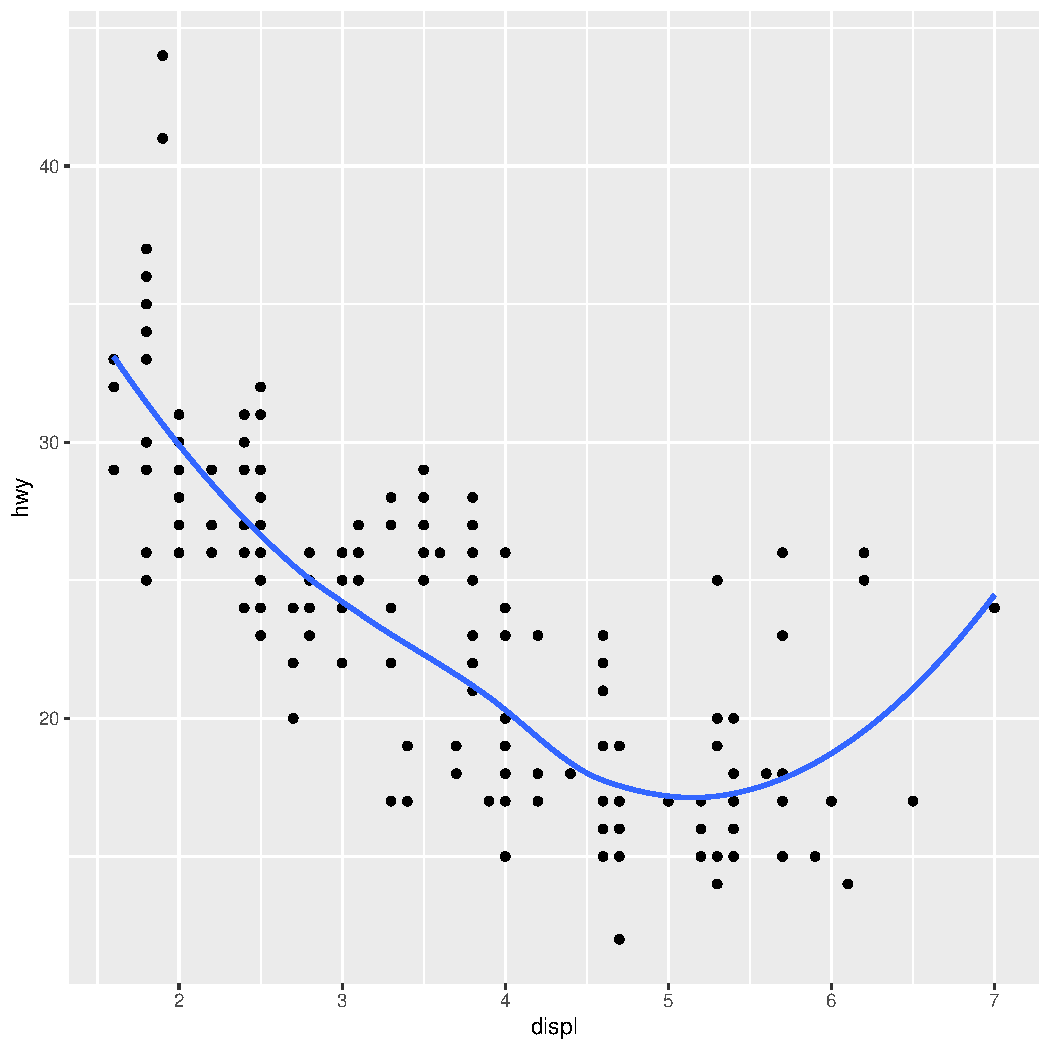
\includegraphics[width=\maxwidth]{figure/unnamed-chunk-7-1} 
\end{knitrout}
	\end{enumerate}
\end{enumerate}
\end{document}
